\subsection{目标检测概述}
目标检测是计算机视觉领域的一个重要分支,
旨在识别图像或视频中特定目标的位置和类别。
它结合了图像分类和目标定位两项任务,
是许多高级视觉应用(如自动驾驶、智能监控、机器人视觉等)的基础。

\subsection{目标检测算法分类}
目标检测算法大致可以分为两类:
\begin{itemize}
    \item \textbf{两阶段检测器 (Two-stage Detectors)}:
    这类算法首先生成候选区域(Region Proposals),
    然后对这些候选区域进行分类和边界框回归。
    代表算法有R-CNN系列(R-CNN, Fast R-CNN, Faster R-CNN)。
    \item \textbf{单阶段检测器 (One-stage Detectors)}:
    这类算法直接在图像上预测目标的类别和边界框,
    无需生成候选区域。代表算法有YOLO系列、SSD、RetinaNet、FCOS等。
\end{itemize}
\subsection{MMDetection 工具箱}
MMDetection 是一个由 OpenMMLab 开发的开源目标检测工具箱,
它基于 PyTorch 实现。MMDetection 提供了丰富多样的 SOTA (State-of-The-Art) 目标检测算法实现,
包括本文实验中使用的 YOLO 系列、Faster R-CNN 和 FCOS 等。
它采用了模块化的设计,方便用户进行自定义模型的构建和实验。
MMDetection 工具箱为目标检测的研究和应用提供了高效灵活的平台,
极大地促进了算法的复现和性能评估。

\subsection{YOLO系列算法}
YOLO (You Only Look Once) 系列算法是单阶段目标检测器的典型代表,以其速度快、实时性好而闻名。
YOLOv3引入了多尺度预测、Darknet-53骨干网络和FPN(Feature Pyramid Network)结构,显著提升了检测精度。
YOLOv5在YOLOv3的基础上进行了多项优化,包括Mosaic数据增强、自适应锚框计算、Focus结构等,进一步提升了性能和易用性。
YOLOv8是Ultralytics公司推出的最新版本,在模型结构、损失函数和训练策略上进行了改进,提供了更快的速度和更高的精度。
图1描述了YOLOv8的网络架构。
\begin{figure}[h!]
    \centering
    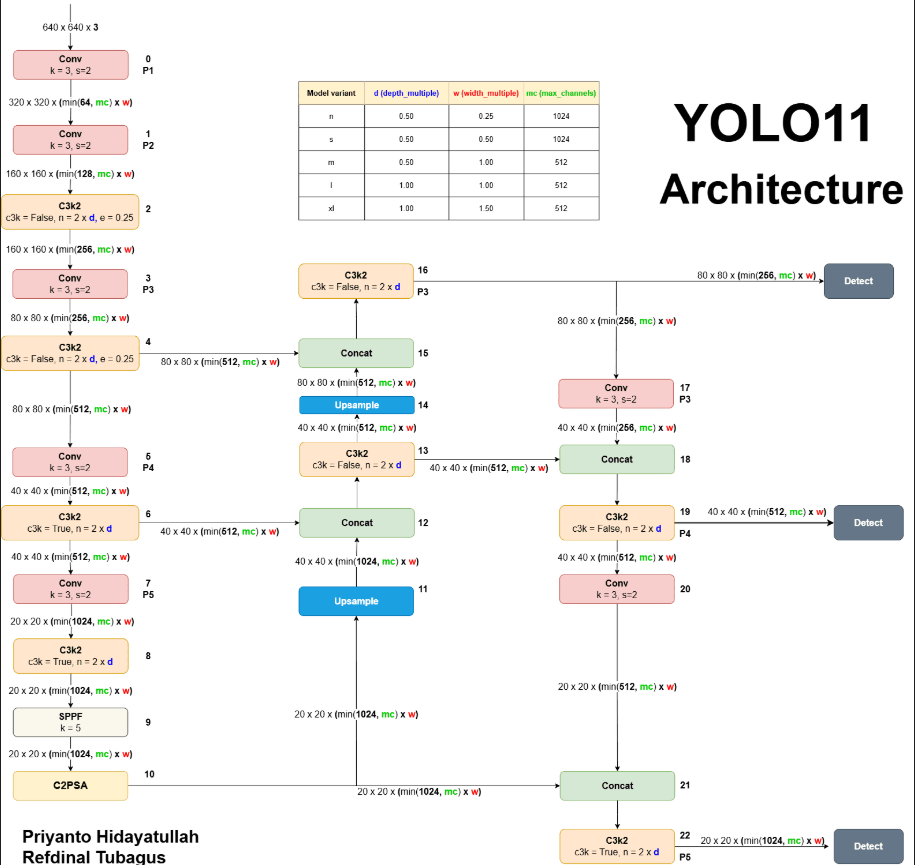
\includegraphics[width=\textwidth]{imgs/yolo11-architecture}
    \caption{YOLOv8 网络结构示意图}
    \label{图1:}
\end{figure}

\subsection{Faster R-CNN}
Faster R-CNN是两阶段检测器的代表,由Ren等人于2015年提出。
它通过引入区域候选网络(Region Proposal Network, RPN)实现了端到端的训练,极大地提升了检测速度。
RPN是一个全卷积网络,用于预测目标边界框和目标得分,从而生成高质量的候选区域。
RoI Pooling将不同大小的候选区域映射到固定大小的特征图上,以便后续的全连接层进行分类和回归。
图2描述了Faster R-CNN的网络架构图。
\begin{figure}[h!]
    \centering
    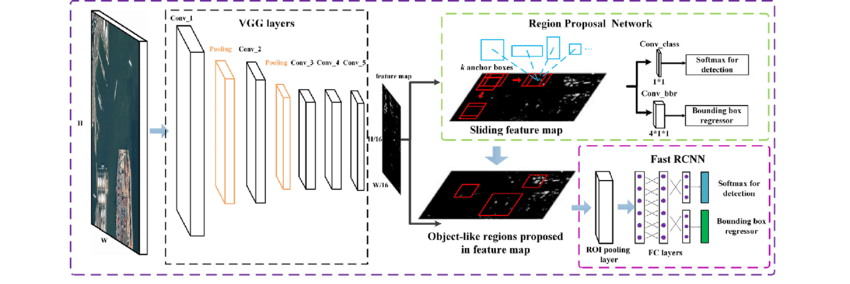
\includegraphics[width=\textwidth]{imgs/The-architecture-of-Faster-R-CNN}
    \caption{Faster R-CNN 网络结构示意图}
    \label{图2:}
\end{figure}